\documentclass[11pt,a4paper]{article}

\usepackage[T1]{fontenc}
\usepackage[utf8]{inputenc}
\usepackage[italian]{babel}
\usepackage{amsmath,amssymb}
\usepackage[a4paper,margin=2.5cm]{geometry}
\usepackage{array}
\usepackage{siunitx}
\usepackage{booktabs}
\usepackage{graphicx}
\usepackage{float}
\usepackage{hyperref}

\hypersetup{hidelinks}
\setlength{\parindent}{0pt}
\setlength{\parskip}{4pt}
\allowdisplaybreaks
\graphicspath{{figure/}}
\sisetup{output-decimal-marker={,}, group-separator={\,}, per-mode=symbol,
         exponent-product=\cdot, range-phrase={\text{--}}}

\newcommand{\uma}{u-a}
\newcommand{\upa}{u+a}

\title{Gasdinamica -- Svolgimento esercizio 1\\[2pt]
\large Svuotamento di un tubo chiuso attraverso un orifizio: pressione sulla parete di testa}
\author{}
\date{Prova del 14/09/2026}

\begin{document}
\maketitle

\section*{Traccia}
Determinare la storia nel tempo della pressione sulla parete di testa del serbatoio dopo l'apertura del setto e
fino al raggiungimento delle condizioni di flusso subsonico in uscita. Fornire il grafico pressione--tempo. Le
condizioni iniziali sono: $P_{tot}=\SI{10}{atm}$, $T_{tot}=\SI{293.15}{K}$ e $P_{amb}=\SI{1}{atm}$.
Figura: condotto di sezione $A_1$ e lunghezza $L=\SI{10}{m}$, chiuso a sinistra, che termina a destra con la
sezione $A_2$, $A_2/A_1=\num{0.506}$, chiusa dal setto.

%==============================================================================
\section{Lettura del testo e dati}
\begin{figure}[H]
  \centering
  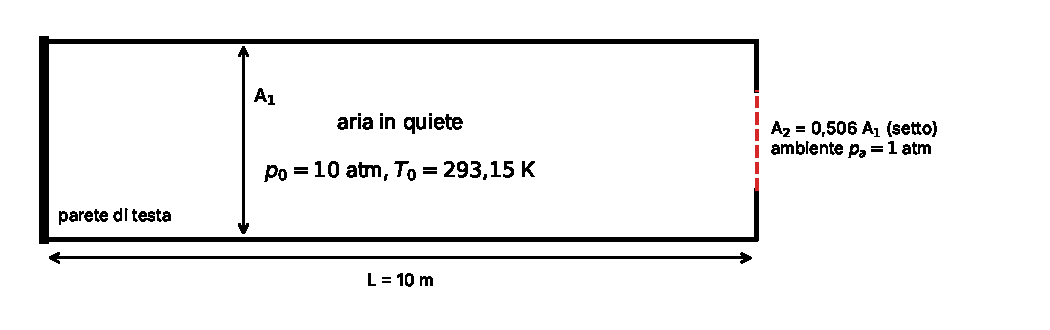
\includegraphics[width=0.85\textwidth]{schema.pdf}
  \caption{Schema del serbatoio (non in scala).}
\end{figure}
Il ``serbatoio'' è il condotto stesso: un tubo di sezione costante $A_1$, lungo \SI{10}{m}, chiuso a sinistra
dalla parete di testa e terminato a destra da un restringimento brusco alla sezione $A_2$, dove si trova il setto.
Il gas è in quiete, quindi le grandezze totali assegnate coincidono con quelle statiche. La traccia non indica il
gas: assumo \textbf{aria}. L'area $A_1$ non serve, conta solo il rapporto $A_2/A_1$.

\begin{table}[H]
  \centering
  \begin{tabular}{lll}
    \toprule
    Grandezza & Valore & Note \\
    \midrule
    $\gamma$, $R$ & \num{1.4}, \SI{287}{J/(kg.K)} & aria (ipotesi); $\delta=(\gamma-1)/2=\num{0.2}$ \\
    $p_0$, $T_0$ & \SI{10}{atm}, \SI{293.15}{K} & stato 0, gas in quiete \\
    $a_0=\sqrt{\gamma R T_0}$ & \SI{343.2}{m/s} & \\
    $p_a$ & \SI{1}{atm} & ambiente \\
    $L$, $A_2/A_1$ & \SI{10}{m}, \num{0.506} & \\
    \bottomrule
  \end{tabular}
  \caption{Dati del problema.}
\end{table}
Si chiede $p(x=0,t)$ dall'apertura del setto ($t=0$) all'istante $t_u$ in cui l'efflusso da $A_2$ smette di
essere critico.

%==============================================================================
\section{Modello e ipotesi}
\begin{itemize}
\item \textbf{Eulero 1D instazionario} nel tubo a sezione costante, gas perfetto, non viscoso e adiabatico, con
  onde piane. Trascuro attrito e scambio termico con le pareti, anche se il tubo è lungo \SI{10}{m}.
\item \textbf{Restringimento brusco} di lunghezza nulla: il gas lo attraversa in un tempo nullo rispetto ai tempi
  delle onde nel tubo. Lo tratto quindi come un collegamento stazionario e isentropico fra la sezione terminale del
  tubo e $A_2$, con portata, $h_0$ ed $s$ conservate e legge delle aree. Il flusso nel convergente accelera, quindi
  l'ipotesi isentropica è ragionevole.
\item \textbf{Flusso omoentropico}: lo stato iniziale è uniforme e, come si vede nell'analisi qualitativa, nascono
  solo espansioni. Allora $R_1=a-\delta u$ si conserva lungo le $\uma$ e $R_2=a+\delta u$ lungo le $\upa$, in tutto
  il campo, comprese le zone d'interazione.
\item Apertura istantanea del setto. Il problema del getto esterno (urto di avviamento, contatto e getto
  sottoespanso) non serve, perché finché $A_2$ è sonica il tubo non riceve informazioni dall'esterno.
\item Non uso $p_0$ e $T_0$ costanti nel tubo (problema instazionario). Il modello a parametri concentrati per lo
  svuotamento lo uso solo come confronto.
\end{itemize}

%==============================================================================
\section{Analisi qualitativa}
All'apertura del setto la pressione esterna è molto minore di quella interna: dall'estremo destro parte
un'\textbf{espansione centrata della famiglia $\uma$} (verso sinistra) che mette il gas in moto verso
l'uscita (l'espansione richiama il fluido nel verso opposto a quello in cui si propaga).

\textbf{Condizione d'uscita.} Il rapporto $p_a/p_0=\num{0.1}$ è molto inferiore al valore critico
$(2/(\gamma+1))^{\gamma/(\gamma-1)}=\num{0.528}$, quindi mi aspetto $A_2$ \textbf{sonica}. Allora il Mach nella
sezione terminale del tubo non dipende dall'ambiente ma solo da $A_1/A_2$: la legge delle aree dà un valore
subsonico $M_e$. L'espansione si ferma dove $u=M_ea$, la coda resta nel tubo (pendenza negativa) e il
condotto, a sezione costante, non arriva a $M=1$: è il restringimento che strozza la corrente. Questa ipotesi va
verificata a posteriori.

\textbf{Riflessioni.} Sulla \textbf{parete} ($u=0$) l'espansione si riflette con la stessa natura: espansione
$\upa$. Quando questa arriva all'\textbf{uscita strozzata}, il vincolo $u=M_ea$ fa sì che anche lì la riflessa sia
un'espansione (della famiglia $\uma$): con $M_e$ piccolo l'orifizio si comporta quasi come un estremo chiuso, non
come un estremo aperto a pressione costante, che rifletterebbe una compressione. Il serbatoio si svuota quindi per
\textbf{espansioni successive}, riflesse avanti e indietro, ognuna più debole della precedente. Mi aspetto sulla
parete una storia \textbf{a gradini}: pressione costante (plateau) finché non arriva un ventaglio, poi una discesa
continua, poi un nuovo plateau.

\textbf{Fine dello strozzamento.} Ogni arrivo all'uscita abbassa la pressione totale dello stato di uscita.
Quando $p^*$ in $A_2$ scende sotto $p_a$ l'orifizio smette di essere critico e la condizione al contorno cambia:
lì termina il tratto richiesto.

%==============================================================================
\section{Topologia del campo}
Numero gli stati uniformi: pari quelli a parete (gas fermo), dispari quelli all'uscita (gas con $M=M_e$).

\begin{table}[H]
  \centering
  \small
  \begin{tabular}{clp{8.6cm}}
    \toprule
    Stato & Dove & Onda che lo separa dal precedente \\
    \midrule
    0 & tutto il tubo, $t<0$ & -- \\
    1 & uscita, $u_1=M_ea_1$ & espansione centrata $\uma$ in $(x,t)=(L,0)$ \\
    2 & parete, $u_2=0$ & riflessione a parete: espansione $\upa$ \\
    3 & uscita, $u_3=M_ea_3$ & riflessione all'uscita strozzata: espansione $\uma$ \\
    4 & parete, $u_4=0$ & seconda riflessione a parete: espansione $\upa$ \\
    \bottomrule
  \end{tabular}
  \caption{Stati di plateau fino alla fine dello strozzamento.}
\end{table}
Nel piano $x$--$t$ (fig.~\ref{fig:xt}) si alternano zone uniformi (nessuna famiglia attiva), onde semplici (una
famiglia, caratteristiche rettilinee) e \textbf{zone d'interazione} a due famiglie vicino alla parete e
all'uscita, dove ogni ventaglio si sovrappone alla propria riflessa e le caratteristiche si curvano. Le teste
dei ventagli che entrano in una zona uniforme sono rette; la testa dell'espansione incidente arriva a parete
attraverso il gas in quiete, alla velocità $-a_0$.

%==============================================================================
\section{Scorciatoie fisiche}
Le condizioni ai due estremi sono lineari negli invarianti. A parete $u=0$ dà $R_1=R_2=a$. All'uscita $u=M_ea$
dà $R_1=a(1-\delta M_e)$ e $R_2=a(1+\delta M_e)$, cioè $R_1=r\,R_2$ con $r=(1-\delta M_e)/(1+\delta M_e)$. Allora
gli stati di plateau si ottengono \textbf{senza iterare e senza seguire le zone d'interazione}: a ogni andata e
ritorno $a$ a parete si moltiplica per $r$ e la pressione per $r^{2\gamma/(\gamma-1)}$. Il reticolo delle
caratteristiche serve solo per gli \emph{istanti} e per l'andamento dentro i ventagli.

%==============================================================================
\section{Calcolo}

\subsection*{Stato 1: uscita strozzata}
Con $A_2$ sonica, $A_1/A^*=A_1/A_2=\num{1.976}$. Dalla legge delle aree, ramo subsonico (il gas nel tubo parte
da fermo e accelera solo fino al restringimento):
\[
\frac{A}{A^*}=\frac1{M_e}\left[\frac{2}{\gamma+1}\left(1+\delta M_e^2\right)\right]^{\frac{\gamma+1}{2(\gamma-1)}}
=\num{1.976}\quad\Rightarrow\quad M_e=\num{0.310}.
\]
Le incognite di 1 sono $a_1,u_1$ (la pressione segue dall'isentropica): due equazioni, l'invariante uniforme
dell'onda semplice $\uma$ e la condizione d'uscita.
\[
a_1+\delta u_1=a_0,\quad u_1=M_ea_1\ \Rightarrow\
a_1=\frac{a_0}{1+\delta M_e}=\frac{\num{343.2}}{\num{1.062}}=\SI{323.2}{m/s},\qquad u_1=\SI{100.2}{m/s},
\]
\[
p_1=p_0\left(\frac{a_1}{a_0}\right)^{\frac{2\gamma}{\gamma-1}}=10\cdot\num{0.9416}^{7}=\SI{6.56}{atm},
\qquad T_1=T_0\left(\frac{a_1}{a_0}\right)^2=\SI{260}{K}.
\]
Fronti dell'espansione incidente: testa $dx/dt=-a_0=\SI{-343.2}{m/s}$, coda $u_1-a_1=\SI{-223.0}{m/s}$.

Controllo della condizione d'uscita: lo stato 1 ha pressione totale (locale, quasi stazionaria nel
restringimento)
\[
p_{0,1}=p_1\left(1+\delta M_e^2\right)^{\frac{\gamma}{\gamma-1}}=\SI{7.02}{atm},\qquad
p^*=\num{0.528}\,p_{0,1}=\SI{3.71}{atm}>p_a=\SI{1}{atm}:
\]
$A_2$ è sonica, come ipotizzato, e fuori dall'orifizio il getto è sottoespanso.

\subsection*{Riflessioni: stati 2, 3, 4}
\[
r=\frac{1-\delta M_e}{1+\delta M_e}=\frac{\num{0.938}}{\num{1.062}}=\num{0.8832},\qquad r^{7}=\num{0.4193}.
\]
\textbf{Stato 2 (parete).} La $\uma$ che arriva porta $R_1=a_1-\delta u_1$; con $u_2=0$:
\[
a_2=a_1-\delta u_1=\SI{303.1}{m/s}=r\,a_0,\qquad p_2=p_0\,r^{7}=\SI{4.19}{atm},\qquad T_2=\SI{229}{K}.
\]
\textbf{Stato 3 (uscita).} La $\upa$ che arriva porta $R_2=a_2$; con $u_3=M_ea_3$:
\[
a_3=\frac{a_2}{1+\delta M_e}=\SI{285.4}{m/s},\quad u_3=\SI{88.5}{m/s},\quad p_3=p_1\,r^{7}=\SI{2.75}{atm}.
\]
\textbf{Stato 4 (parete).} $a_4=a_3(1-\delta M_e)=r\,a_2=\SI{267.7}{m/s}$, $\ p_4=p_0\,r^{14}=\SI{1.76}{atm}$,
$\ T_4=\SI{178}{K}$.

\subsection*{Fine dello strozzamento}
L'orifizio resta critico finché $p^*\ge p_a$, cioè finché lo stato nella sezione terminale del tubo (sempre con
$M=M_e$) ha
\[
p_e\ \ge\ \frac{p_a}{\num{0.528}\,(1+\delta M_e^2)^{\gamma/(\gamma-1)}}
=\frac{1}{\num{0.528}\cdot\num{1.069}}=\SI{1.77}{atm},
\]
cioè pressione totale d'uscita di almeno \SI{1.89}{atm}.
Gli stati d'uscita dei plateau sono $p_1=\num{6.56}$ e $p_3=\SI{2.75}{atm}$, entrambi strozzati. Il plateau
successivo avrebbe $p_5=p_3\,r^7=\SI{1.15}{atm}<\SI{1.77}{atm}$: lo strozzamento finisce \emph{durante} l'arrivo
all'uscita della seconda espansione riflessa dalla parete (quella che porta la parete da 2 a 4). In quel momento
la parete è già nello stato 4, perché la riflessione successiva parte dall'uscita e non ha ancora percorso il tubo.

\subsection*{Istanti: reticolo delle caratteristiche}
Divido il ventaglio incidente in tre onde di uguale ampiezza, $\Delta u=u_1/3=\SI{33.4}{m/s}$, cioè quattro
caratteristiche $\uma$ con $R_1=\num{343.2}$, \num{329.8}, \num{316.5}, \SI{303.1}{m/s} (nel ventaglio
$R_2=a_0$). Ciascuna, riflessa a parete, diventa una $\upa$ con $R_2$ uguale al suo $R_1$. All'uscita una
$\upa$ con $R_2$ diventa una $\uma$ con $R_1=r R_2$. Nel nodo in cui la $\uma$ $i$ incontra la $\upa$ $j$ lo
stato è noto subito:
\[
a=\frac{R_{1,i}+R_{2,j}}{2},\qquad u=\frac{R_{2,j}-R_{1,i}}{2\delta}.
\]
La posizione del nodo P si trova dai nodi precedenti A (sulla $\uma$) e B (sulla $\upa$), con le pendenze
medie sui due lati:
\[
x_P-x_A=\tfrac12\left[(u-a)_A+(u-a)_P\right](t_P-t_A),\qquad
x_P-x_B=\tfrac12\left[(u+a)_B+(u+a)_P\right](t_P-t_B).
\]
\emph{Esempio}, primo nodo dopo la parete. La testa riflessa parte da $(0;\ \SI{29.14}{ms})$, perché
$t=L/a_0=\SI{29.14}{ms}$, e incontra la seconda caratteristica del ventaglio, che parte dal centro con
$u-a=\SI{-303.1}{m/s}$. Nel nodo $a=\SI{336.5}{m/s}$, $u=\SI{33.4}{m/s}$, quindi la $\upa$ ha pendenza media
$(343{,}2+369{,}9)/2=\SI{356.6}{m/s}$:
\[
10-303{,}1\,t=356{,}6\,(t-0{,}02914)\ \Rightarrow\ t=\SI{30.9}{ms},\ x=\SI{0.63}{m},\ p=\SI{8.72}{atm}.
\]
Proseguendo allo stesso modo si ottengono gli arrivi a parete e all'uscita (tab.~\ref{tab:nodi}).

\begin{table}[H]
  \centering
  \small
  \begin{tabular}{ccc@{\qquad}ccc}
    \toprule
    \multicolumn{3}{c}{Parete di testa ($u=0$)} & \multicolumn{3}{c}{Uscita del tubo ($u=M_ea$)} \\
    $t$ [ms] & $a$ [m/s] & $p$ [atm] & $t$ [ms] & $a$ [m/s] & $p$ [atm] \\
    \midrule
    0--\num{29.14} & \num{343.2} & 10 (stato 0) & 0--\num{53.3} & \num{323.2} & \num{6.56} (stato 1) \\
    \num{32.9} & \num{329.8} & \num{7.57} & \num{59.2} & \num{310.6} & \num{4.97} \\
    \num{37.5} & \num{316.5} & \num{5.67} & \num{66.4} & \num{298.0} & \num{3.72} \\
    \num{43.3}--\num{87.8} & \num{303.1} & \num{4.19} (stato 2) & \num{75.1}--\num{115.9} & \num{285.4} & \num{2.75} (stato 3) \\
    \num{97.3} & \num{291.3} & \num{3.18} & \num{127.4} & \num{274.3} & \num{2.08} \\
    \num{108.6} & \num{279.5} & \num{2.38} & $\approx\num{135}$ & \num{268.0} & \num{1.77} (fine strozz.) \\
    \num{122.1}--$t_u$ & \num{267.7} & \num{1.76} (stato 4) & & & \\
    \bottomrule
  \end{tabular}
  \caption{Arrivi delle caratteristiche (reticolo con il ventaglio diviso in tre onde).}
  \label{tab:nodi}
\end{table}
L'istante di fine strozzamento si ottiene interpolando fra gli ultimi due nodi d'uscita il valore
$p_e=\SI{1.77}{atm}$: $t_u\approx\SI{135}{ms}$.

Dentro un ventaglio, il valore a parete è fissato dall'invariante della caratteristica che arriva:
$p_w(t)=p_0\,(R_1/a_0)^{7}$. La discesa è più ripida all'inizio, perché le caratteristiche della testa del
ventaglio sono più veloci e più ravvicinate.

%==============================================================================
\section{Verifiche a posteriori}
\begin{itemize}
\item Uscita strozzata all'apertura: $p^*=\SI{3.71}{atm}>p_a$. \textbf{Verificata}.
\item Portata: $\rho_1u_1A_1$ coincide con la portata critica di $A_2$ calcolata con $p_{0,1}$ e $T_{0,1}$
  (\SI{893}{kg/(s.m^2)} per unità di $A_1$). \textbf{Verificata}.
\item Coda dell'espansione incidente: $u_1-a_1=\SI{-223}{m/s}<0$, resta nel tubo, che non raggiunge $M=1$.
  \textbf{Verificata}.
\item Natura delle onde: ogni onda abbassa $R_1$ o $R_2$, quindi sono tutte espansioni. Nel reticolo le
  caratteristiche della stessa famiglia divergono e non si incrociano, quindi non si formano urti e l'ipotesi
  omoentropica regge. \textbf{Verificata}.
\item Condizioni al contorno: nel tubo $0\le u\le M_ea<a$. A parete entra una sola caratteristica ($\upa$) e
  impongo una sola condizione ($u=0$). All'uscita subsonica entra solo la $\uma$ e impongo una sola condizione
  ($M=M_e$). \textbf{Verificata}.
\item Strozzamento fino a $t_u$: $p_1$ e $p_3$ sono maggiori di \SI{1.77}{atm}, $p_5$ minore.
  \textbf{Verificata}: il tratto richiesto termina a $t_u\approx\SI{135}{ms}$.
\item $a>0$ e $p>0$ ovunque (minimo $a_4=\SI{268}{m/s}$): nessun vuoto. \textbf{Verificata}.
\end{itemize}

%==============================================================================
\section{Risultati}
\begin{table}[H]
  \centering
  \small
  \begin{tabular}{llll}
    \toprule
    Intervallo [ms] & $p$ sulla parete di testa & Causa & Valore \\
    \midrule
    $0\le t\le\num{29.1}$ & $p=\SI{10}{atm}$ (stato 0) & la testa $\uma$ non è arrivata & esatto \\
    $\num{29.1}$--$\num{43.3}$ & da 10 a \SI{4.19}{atm} & espansione incidente + riflessa & istanti stimati \\
    $\num{43.3}$--$\num{87.8}$ & $p_2=p_0r^7=\SI{4.19}{atm}$ & plateau & esatto \\
    $\num{87.8}$--$\num{122}$ & da \num{4.19} a \SI{1.76}{atm} & espansione riflessa dall'uscita & istanti stimati \\
    $\num{122}$--$t_u$ & $p_4=p_0r^{14}=\SI{1.76}{atm}$ & plateau & esatto \\
    \bottomrule
  \end{tabular}
  \caption{Storia della pressione sulla parete di testa fino alla fine dello strozzamento.}
\end{table}
Altri risultati: $M_e=\num{0.310}$; $p_1=\SI{6.56}{atm}$, $u_1=\SI{100}{m/s}$; fine dell'efflusso critico a
$t_u\approx\SI{135}{ms}$, con pressione d'uscita \SI{1.77}{atm} e pressione a parete \SI{1.76}{atm}. I valori dei
plateau sono esatti nel modello; gli istanti dentro le zone d'interazione vengono dal reticolo delle
caratteristiche.

%==============================================================================
\section{Rappresentazioni}
\begin{figure}[H]
  \centering
  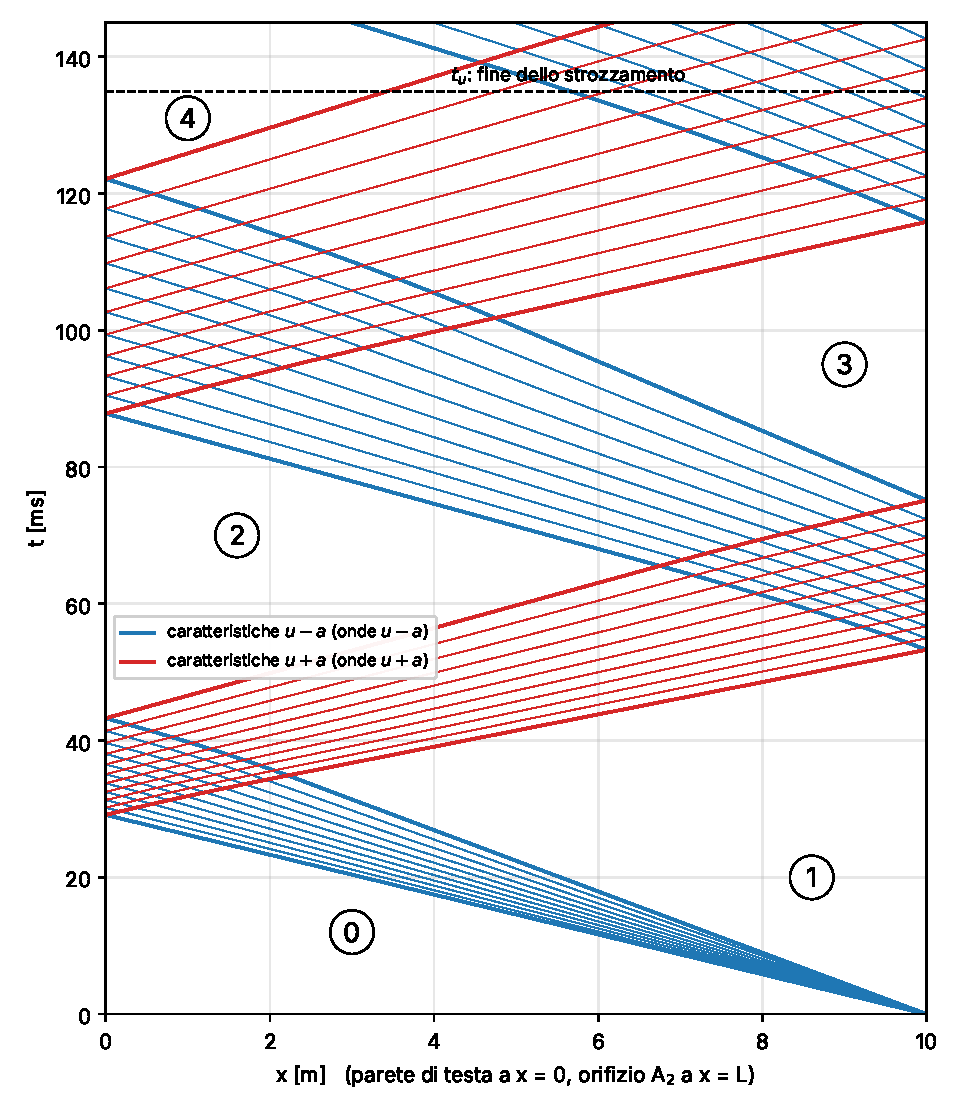
\includegraphics[width=0.70\textwidth]{xt.pdf}
  \caption{Piano $x$--$t$: caratteristiche $\uma$ (blu) e $\upa$ (rosse); le linee spesse sono teste e code dei
  ventagli. Gli stati di plateau sono numerati.}
  \label{fig:xt}
\end{figure}
\textbf{Piano $x$--$t$} (fig.~\ref{fig:xt}). Il ventaglio incidente è centrato in $(L,0)$ ed è stretto (la coda
viaggia a \SI{-223}{m/s}). Arrivando a parete forma la prima zona d'interazione (29--\SI{43}{ms}), dove le
caratteristiche si curvano. Ne esce la riflessa $\upa$, che è più larga perché le sue caratteristiche viaggiano a
velocità diverse ($u+a$ da \num{423} a \SI{303}{m/s}). All'uscita (53--\SI{75}{ms}) nasce la seconda zona
d'interazione e la nuova $\uma$, più larga ancora, impiega circa \SI{34}{ms} a passare la parete. I ventagli si
allargano a ogni passaggio, quindi i plateau si accorciano. A $t_u$ la testa della terza espansione ha appena
lasciato l'uscita e non ha ancora raggiunto la parete, che quindi resta nello stato 4.

\begin{figure}[H]
  \centering
  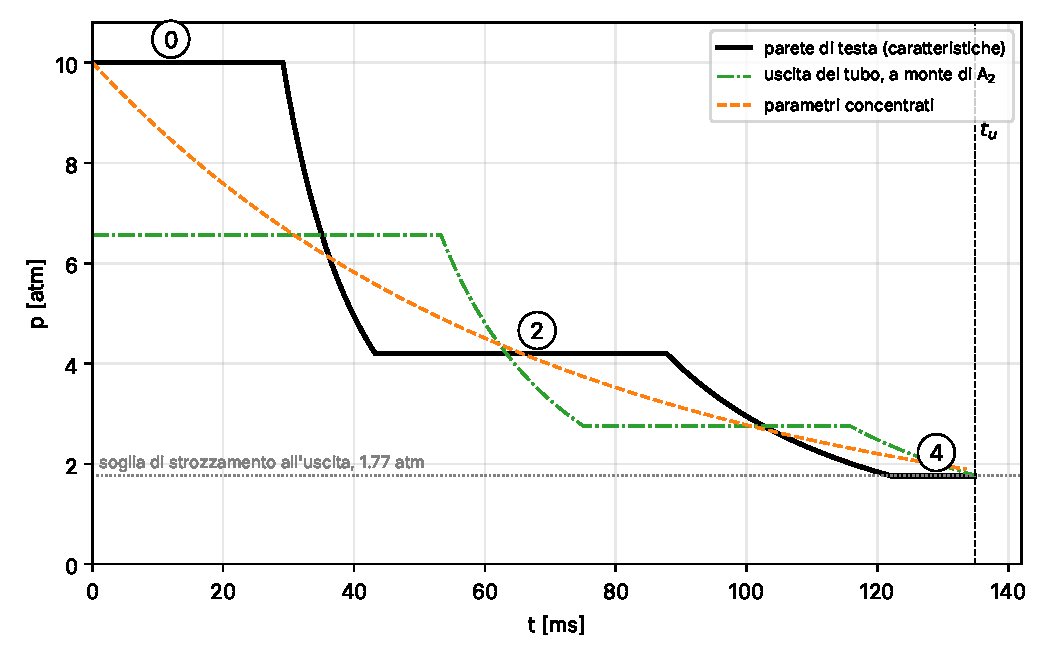
\includegraphics[width=0.85\textwidth]{p_t.pdf}
  \caption{Pressione sulla parete di testa (nero), nella sezione terminale del tubo (verde) e secondo il modello
  a parametri concentrati (arancio), fino a $t_u$.}
  \label{fig:pt}
\end{figure}
\textbf{Grafico pressione--tempo} (fig.~\ref{fig:pt}, richiesto dalla traccia). È tracciato infittendo il
reticolo delle caratteristiche; i punti della tab.~\ref{tab:nodi} cadono sulla curva. La parete resta a
\SI{10}{atm} per $L/a_0$, poi scende a gradini: a ogni ventaglio la pressione si moltiplica per $r^7=\num{0.42}$.
La curva dell'uscita è sfasata di circa mezzo periodo e scende per prima, dato che le espansioni partono da lì.
Le pressioni vanno da 10 a \SI{1.8}{atm}, meno di un ordine di grandezza, quindi basta la scala lineare.

\begin{figure}[H]
  \centering
  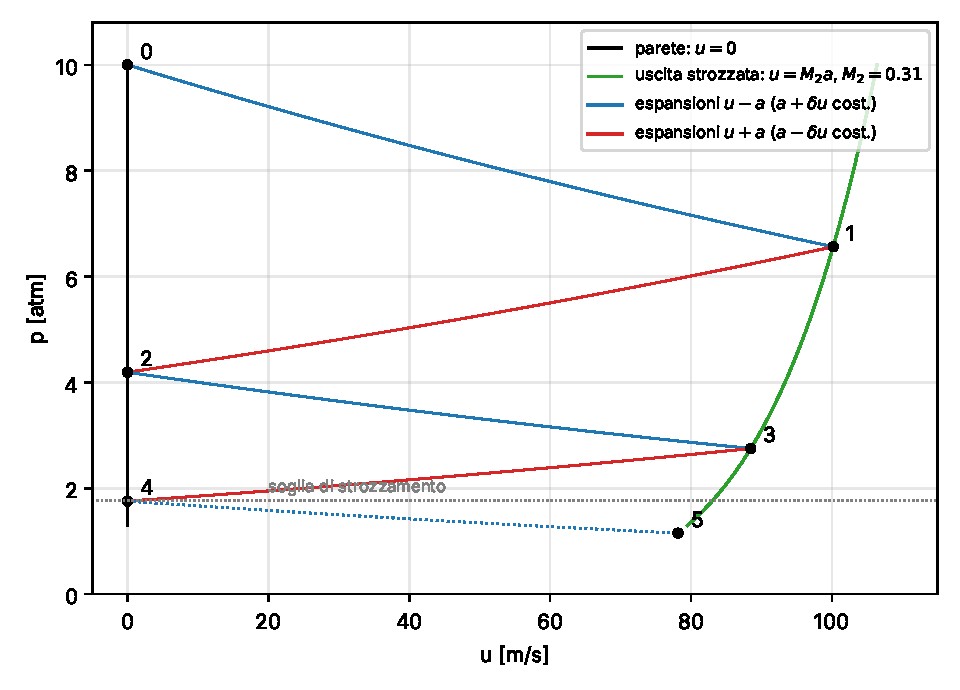
\includegraphics[width=0.70\textwidth]{p_u.pdf}
  \caption{Piano $p$--$u$: gli stati di plateau rimbalzano fra la retta di parete $u=0$ e la curva d'uscita
  $u=M_ea$ lungo le curve delle onde semplici. Lo stato 5 (tratteggiato) non viene raggiunto in regime strozzato.}
  \label{fig:pu}
\end{figure}
\textbf{Piano $p$--$u$} (fig.~\ref{fig:pu}). Ogni plateau sta su una delle due curve di contorno: gli stati pari
sull'asse $u=0$, i dispari sulla curva $u=M_ea$, che passa per l'origine perché $a$ scende con $p$. Si passa
dall'una all'altra lungo le curve di espansione $\uma$ ($a+\delta u$ costante) e $\upa$ ($a-\delta u$
costante). È una ``scala'' che scende verso l'origine e mostra perché il serbatoio non si svuota in un solo
passaggio: ogni riflessione toglie solo una frazione della pressione. La retta orizzontale a \SI{1.77}{atm}
separa gli stati d'uscita strozzati da quelli che non lo sono più.

%==============================================================================
\section{Discussione fisica}
\begin{itemize}
\item \textbf{Ruolo dell'orifizio.} Senza restringimento ($A_2=A_1$) l'espansione verso $p_a=0{,}1\,p_0$ sarebbe
  transonica con uscita sonica, e il tubo si svuoterebbe molto più in fretta. Con $A_2/A_1=\num{0.506}$ il
  gas nel tubo esce a $M_e=\num{0.31}$ e l'orifizio riflette le espansioni quasi come una parete (coefficiente
  $r=\num{0.88}$ sugli invarianti, contro 1 della parete e $-1$ di un estremo aperto in acustica). Per questo
  la pressione scende a gradini e non in modo continuo.
\item \textbf{Riflessione a parete.} Il primo salto a parete (da 10 a \SI{4.19}{atm}) è molto maggiore di
  quello dell'onda incidente (da 10 a \SI{6.56}{atm}): incidente e riflessa si sommano, come il raddoppio
  dell'ampiezza nel limite acustico. Il raddoppio non è esatto perché l'onda è finita.
\item \textbf{Confronto con il modello a parametri concentrati.} Con $V=A_1L$ e orifizio critico
  $A_2$: $K=A_2a_0C_*/V=\SI{10.0}{s^{-1}}$ con $C_*=\num{0.579}$, e
  $p/p_0=[1+\delta Kt]^{-7}$. Questo modello dà una discesa continua e la fine dello strozzamento a
  $p=\SI{1.89}{atm}$ per $t\approx\SI{134}{ms}$. Il tempo di svuotamento $1/K\approx\SI{100}{ms}$ è dello stesso
  ordine del tempo acustico $2L/a_0=\SI{58}{ms}$, quindi l'ipotesi di serbatoio uniforme non vale e la storia a
  parete è quella a gradini. Il bilancio di massa globale però è lo stesso, e infatti la curva a parametri
  concentrati passa in mezzo ai gradini e prevede $t_u$ quasi uguale (\num{134} contro \SI{135}{ms}).
\item \textbf{Temperature.} L'espansione è isentropica: a parete $T$ scende fino a \SI{178}{K} in \SI{0.12}{s}.
  Nella realtà lo scambio termico con le pareti e l'attrito, su un tubo di \SI{10}{m}, smorzerebbero i gradini e
  rallenterebbero il raffreddamento. Se l'aria è umida si può avere condensazione.
\item \textbf{Dopo $t_u$.} L'orifizio non è più critico: all'uscita si impone $p=p_a$ nella sezione $A_2$ e la
  condizione al contorno diventa simile a quella di un estremo aperto. Le espansioni che arrivano non si
  riflettono più come espansioni ma tendono a riflettersi come compressioni. La pressione tende a $p_a$ con
  oscillazioni smorzate, ma questa fase non è richiesta.
\end{itemize}

\end{document}
